Regarding image transforms, one of the most important examples is the Fourier Transform. It was conceived by Jean Baptiste Joseph Fourier (1768 - 1830) and basically states that any periodic function can be expressed as the sum of sines and cosines of different frequencies, each multiplied by a different coefficient \cite{gonzalez2018digital}. According to \citeonline{brigham1988fast}, the relationship between the different frequency sinusoids and arbitrary function $s$ to be analyzed is described as

\begin{equation}
\label{eqn:fourier_transform}
S(f) = \int_{-\infty}^{\infty}s(x)e^{-j 2 \pi f x} dx,
\end{equation}

\noindent where $S(f)$ is the Fourier Transform of the $s(t)$ and $j = \sqrt{-1}$ represents the imaginary unit. Note that the function transformed from the one-dimensional spatial domain to the frequency domain, represented by $f$. Similarly, the inverse transform is denoted by

\begin{equation}
\label{eqn:inverse_fourier_transform}
s(x) = \int_{-\infty}^{\infty}S(f)e^{j 2 \pi f x} df.
\end{equation}

As stated by \citeonline{bracewell2000fourier}, an arbitrary periodic function $s$ with period $T$ is commonly to express it as a Fourier series, given by the expression

\begin{equation}
\label{eqn:fourier_series}
a_{0} + \sum_{1}^{\infty} (a_{n} \cos{2 \pi n f t} + b_{n} \sin{2 \pi n f t}),
\end{equation}

\noindent where

\begin{align*}
a_{0} &= \frac{1}{T} \int_{-\frac{1}{2} T}^{\frac{1}{2} T} s(t) dt\\
a_{n} &= \frac{2}{T} \int_{-\frac{1}{2} T}^{\frac{1}{2} T} s(t) \cos{(2 \pi n f t)} dt\\
b_{n} &= \frac{2}{T} \int_{-\frac{1}{2} T}^{\frac{1}{2} T} s(t) \sin{(2 \pi n f t)} dt\\
\end{align*}

If the function is not periodic, then the Fourier Transform is applied as a continuous function of frequency, i.e. $s(t)$ is represented by the sum of sinusoids of all frequencies \cite{brigham1988fast}. Particularly, this stands for images, which are non-periodic functions. The common approach is to appraise the image as a section of a periodic function so the use of Fourier Transform makes sense.

The equations \ref{eqn:fourier_transform} and \ref{eqn:inverse_fourier_transform} together are named a \emph{Fourier Transform pair}. Images are represented by two-variable functions, which motivates the use of a two-dimensional Fourier Transform; moreover, as digital images are matrix representations of images, the two-dimensional \sigla{DFT}{Discrete Fourier Transform} is the most relevant brand of the FT for image processing applications. Consequently, the two-dimensional Fourier Transform pair of a function $s(x,y)$ is given by

\begin{align}
\label{eqn:two_dimensional_continuous_fourier_transform}
S(u,v) &= \int_{-\infty}^{\infty}
         \int_{-\infty}^{\infty}
         s(x,y) e^{-j 2 \pi 
                    \left(
                        ux + vy
                    \right)
                  }
        dx dy\\
s(x,y) &= \int_{-\infty}^{\infty}
         \int_{-\infty}^{\infty}
         S(u,v) e^{j 2 \pi 
                    \left(
                        ux + vy
                    \right)
                  }
        du dv.
\end{align}

According to \citeonline{bracewell2000fourier}, this pair of equations represents the analysis of $s(x,y)$ into components of the form $\exp{\left[j 2 \pi (ux + vy) \right]}$, where the variables $u$ and $v$ represent spatial frequencies. The equation that relates such components to sinusoids is the \emph{Euler's Formula} or \emph{Euler's Identity}, written as

\begin{equation}
\label{eqn:euler_formula}
    e^{j\theta} = \cos{\theta} + j\sin{\theta}
\end{equation}

\noindent where $\theta = 2 \pi f$ is a number that represents an angle in radians and $e^{j\theta}$ is the polar form representation of the sinusoids \cite{gonzalez2018digital}. Finally, the common two-dimensional DFT form applied among image processing is, as reported by \citeonline{gonzalez2018digital}, denoted by

\begin{align}
\label{eqn:two_dimensional_discrete_fourier_transform}
S(u,v) &= \sum_{x = 1}^{M}
          \sum_{y = 1}^{N}
          s(x,y) e^{-j 2 \pi 
                    \left(
                        ux/M + vy/
                    \right)
                  }
        dx dy\\
s(x,y) &= \frac{1}{MN}
          \sum_{1}^{M}
          \sum_{1}^{N}
          S(u,v) e^{j 2 \pi 
                    \left(
                        ux/M + vy/N
                    \right)
                  }
        du dv,
\end{align}

\noindent where $s(x,y)$ is a discrete function that represents an image of size $M \times N$, $x$ and $y$, discrete variables that represent spatial coordinates, $u$ and $v$ are discrete spatial frequencies. 

One prominent example of Fourier Transform use is the Convolution Theorem. It states that convolution may be computed by a multiplication in the Fourier domain \cite{brigham1988fast}. This allows much faster computations of convolution in comparison to the spatial domain approach and is frequently used in many applications, such as image filtering and convolutional neural networks. In terms of computational complexity, the common two-dimensional Discrete Fourier Transform implementations yield results in $\mathcal{O}(n^{2})$ time for square or zero-padded images and $\mathcal{O}(mn)$ for images of size $m \times n$; for this reason, the \sigla{FFT}{Fast Fourier Transform} is a divide-and-conquer implementation created by Cooley and Tookey in 1965 and reduces the computational complexity to $\mathcal{O}(n \log n)$ \cite{bracewell2000fourier}. The Fourier Transform is widely employed in this work and the chosen approach to compute it is the FFT algorithm.


% \subsection{Image Fusion}

% Immediately upon the blur map extraction is satisfactorily complete, an image fusion operation is needed in order to achieve the highest amount of focused regions as possible. Image fusion is a process that merges several images (possibly taken in diverse conditions or with different cameras) into one image with higher quality, more details and consequently more useful for humans and computer tasks \cite{mitchell2010image}. Image fusion techniques can be used in noise reduction, edge enhancement and super-resolution, for example. 

% One prominent use of image fusion occurs in medical image fields; the quality of information about illnesses, cells, clinical analysis and several other medical tasks (including the computer assisted ones) have found profitable results from the techniques and lead themselves to better and faster decisions when it comes to human beings \cite{james2014medical}.

% There are relevant applications in remote sensing multispectral images, segmentation of regions in different colourspaces, biometry: the pan-sharpening process is the generation of an high resolution multispectral image from low to high resolution ones, K-Means segmentation and fusion of pixels in the \sigla{RGB}{Red, Green and Blue colourspace} and the Iris Recognition biometric process with video frames are examples of such tasks, respectively \cite{mitchell2010image}.

% \subsection{General Framework}

% Still according to \citeonline{mitchell2010image}, the general framework for the image fusion procedure can be accomplished in four stages: Multiple Input Images, Common Representational Format, Fusion and Display.
% The \emph{multiple input images} stage consists in obtaining the set of images which will be merged. There are several approaches to this: the dataset may be captured from different sensors, on distinct light conditions or angles, with different magnifications, on several focus and with temporal measurements if the scene changes through time.

% After the image set generation, there is the necessity of reshaping each item. This configures the \emph{common representational format}, responsible for creating a new and temporary dataset with the same properties, e.g. colourspace, dimensions, noise level and so on. The \emph{fusion} stage consists of using a decision method in order to dictate which regions, objects, colours or details will compose the final image; this can be done by any approach that relates to how the result should be. There are some methods that rely on the Wavelet Transform domain, for example. Finally, the \emph{display} stage consists in providing a view for the resulting image, which can be used directly for any further task or even be the input for other image processing operation. Figure \ref{fig:fusion_general_framework} depicts an arbitrary example of the four stages:

% \begin{figure}[H]
% 	\centering
% 	\caption{\label{fig:fusion_general_framework}Image fusion general framework. (a) Multiple Input Images, (b) Common Representational Format, (c) Fusion and (d) Display.}
% 	\begin{center}
% a 	    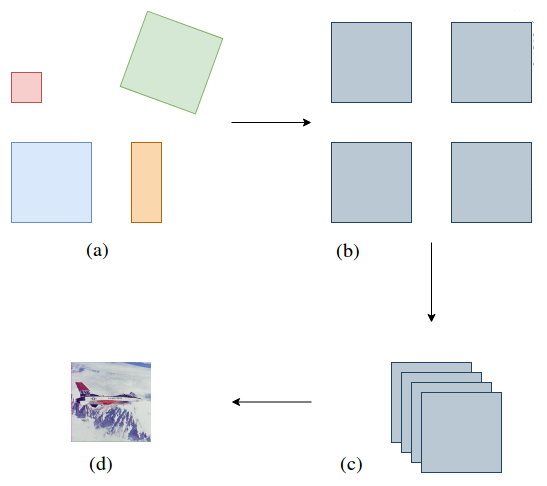
\includegraphics[scale=0.4]{images/fig10.png}
% 	\end{center}
% 	\centering
%     \fautor
% \end{figure}

% The four arbitrary images in Figure \ref{fig:fusion_general_framework}.\textbf{(a)} represents different images of the same scene, taken at different resolutions, rotations and shapes. In \ref{fig:fusion_general_framework}.\textbf{(b)}, the images are all reshaped, converted to the same colourspace and ready to receive processing algorithm which will transform them into feature vectors. Figure \ref{fig:fusion_general_framework}.\textbf{(c)} represents the image fusion by means of an arbitrary method. The resulting image is depicted in Figure \ref{fig:fusion_general_framework}.\textbf{(d)}.

% Since image fusion is only one branch of data fusion field, this procedure has a wide variety approaches and methods; hence, the domain will be restricted to the multifocus image fusion and some related work will be presented as follows, in section \ref{sec:multifocus_image_fusion}.
